%----------------------------------------------------------------------------
\chapter{Evaluation}
%----------------------------------------------------------------------------
\label{chap:evaluation}
%Összesen kb. 5-8 oldal

In the current chapter the environment used for assessing the implementation is introduced in \autoref{sec:meas-workflow}, \autoref{sec:meas-env} and in \autoref{sec:meas-patterns}, then the performance of the implemented local search-based pattern matching algorithm is evaluated in \autoref{sec:performance-evaluation}. An additional measurement was done for scalability in an environment with limited memory in \autoref{sec:performance-evaluation-tb}.

%1-2 oldal
\section{Measurement workflow}
\label{sec:meas-workflow}

The measurement setup is composed of four phases: (i) \emph{Read}, (ii) \emph{Create engine}, (iii) \emph{Calculate search plan}, and (iv) \emph{Check}. The steps are depicted in \autoref{fig:measurement-workflow}. 

\begin{figure}[!htp]
	\centering
	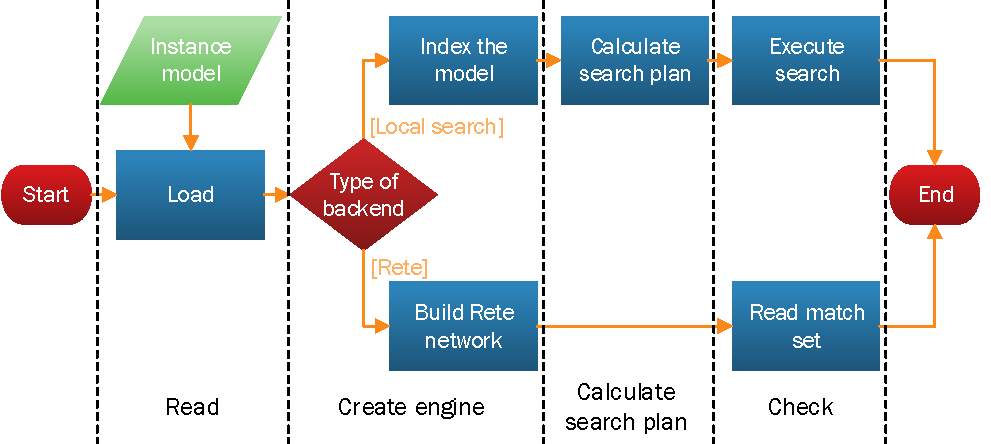
\includegraphics[width=\textwidth]{figures/pdfs/measurement_workflow.pdf}
	\caption{The workflow used for measurements}
	\label{fig:measurement-workflow}
\end{figure}

The Read step measures merely the time needed to load the EMF model into memory. The Create engine step is different for the incremental, and local search-based approaches. For a local search based-algorithm only a basic indexing of the elements is performed in order to provide cardinality information for the search plan calculation. In case of Rete, in addition to the indexing, the whole Rete network is created, which means most of the pattern matching is done here. Calculate search plan phase is only related to local search, for in this step the search plan calculation time is monitored. Finally the time needed for the retrieval of results is observed in the Check phase.


%In this scenario we only assess search execution times executed on a loaded model for the first time. Model modification and re-checking is out of scope, for it means no difference for the local search-based pattern matching.

\section{Measurement environment}
\label{sec:meas-env}

The computer used for carrying out the measurements was a ThinkPad T440p laptop, running Linux 3.16.0-38-generic x86\_64 operating system, and had the following hardware configuration:
\begin{itemize}
	\item CPU: Intel$\circledR$ Core\texttrademark~i7-4700MQ CPU @ 2.40GHz
	\item Memory: 2 $\times$ 4096 MB DDR3 @ 1600 MHz
	\item SSD: Intel 320 Series SSDs, model: INTEL SSDSA2CW160G3
\end{itemize}

We used Java\texttrademark~SE Runtime Environment (build 1.8.0\_66-b17). In order to successfully load every used model to memory, we supplied the JVM 6 gigabytes of heap size by using the \texttt{-Xms6G} and \texttt{-Xmx6G} parameters. 

We tested the performance of the incremental Rete (referred as \emph{Incremental}), the single-threaded local search-based (\emph{Sequential}), and the parallel local search-based (\emph{Parallel}) algorithms. We assessed the performance using the newest algorithm versions available on December 10, 2015 in \eiq.


\section{Models and patterns used for assessment}
\label{sec:meas-patterns}
In order to evaluate scalability of the algorithms, we carried out measurements on three different model sizes with four different queries. Both the models and queries are from~\cite{DBLP:journals/infsof/UjhelyiSHCVVF15}. 

The selected models for this work are the EMF representations of the ASGs of programs \emph{Qwicap}, \emph{Frinika}, and \emph{Hibernate}. Qwicap is a library for Java web application development. Frinika is a music workstation software, which provides several features for editing and working with music. Hibernate is a tool that can be used to implement object-relation mapping for applications to persist data. We chose these softwares, because both are free and open-source, and have different sizes, thus they can help assessing scalability of the approaches. \autoref{tab:model-complexity} summarizes the basic metrics of the source code and the generated ASGs.

% Attributes are not needed for the example queries
%\begin{table}[htbp]
%	\centering
%	\begin{tabular}{c|crrrr}
%		\hline
%		& Version	& LOC		& Node Count 	& Edge Count	& Attribute Count \\
%		\hline
%		
%		Qwicap		 & 1.4b24	& 443 		& 7,903 			& 21,222 		& 59,069 \\			
%		Frinika		 & 0.5.1	& 64,828 	& 429,407 		& 1,292,961 		& 3,065,383 \\		
%		Hibernate	 & 3.5.0	& 773,166 	& 2,444,419 		& 7,563,207 		& 16,789,330 \\	
%		\hline
%	\end{tabular}
%	\caption{Metrics of the analysed ASGs}
%	\label{tab:model-complexity}
%\end{table}

\begin{table}[htbp]
	\centering
	\begin{tabular}{l|crrr}
		\hline
	 Model name& Version	& LOC		& Node Count 	& Edge Count	\\
		\hline

	Qwicap		 & 1.4b24	& 443 		& 7,903 			& 21,222 		\\			
	Frinika		 & 0.5.1	& 64,828 	& 429,407 		& 1,292,961 		\\		
	Hibernate	 & 3.5.0	& 773,166 	& 2,444,419 		& 7,563,207 	\\	
	\hline
	\end{tabular}
	\caption{Metrics of the analyzed ASGs}
	\label{tab:model-complexity}
\end{table}



The four cases if code smell are named \emph{Catch}, which is the same as the example \catchproblem pattern describes, \emph{Constant compare}, \emph{No default switch} and \emph{Unused parameter}. The descriptions of the latter three anti-patterns are again taken from~\cite{DBLP:journals/infsof/UjhelyiSHCVVF15}, and are as follows:

\begin{itemize}
	\item \emph{Constant compare}: When a String variable is compared
	to a String literal using the \texttt{equals()} method, it is unsafe to have the variable
	on the left hand side. Changing the order makes the code safe (by avoiding
	null pointer exception) even if the String variable to compare is \texttt{null}.
	\item \emph{No default switch}: Missing default \texttt{case} has to be added to the \texttt{switch}.
	\item \emph{Unused parameter}: When unused parameters remain in the parameter list
	they can be removed from the source code in most cases.
\end{itemize}

In \autoref{tab:pattern-complexity} we summarized the total number of variables, constraints, and any type of pattern calls used to describe the problem using IQPL. These numbers does not provide precise description, however, they tell that these patterns are adequate for performing measurements to test scalability of the approaches from the aspect of pattern complexity. The \emph{No default switch} is considered to be the simplest, while \emph{Unused parameter} the most difficult to match. 

\begin{table}[!htpb]
	\centering
	\begin{tabular}{l|ccc}
		\hline
 Anti-pattern problem & Variables & Constraints & Pattern calls\\
		\hline
 Catch 			& 6 	& 9 	& 1	\\
 Constant compare & 9 	& 10 	& 4	\\
 No default switch & 3 	& 5 	& 1	\\
 Unused parameter & 19 	& 29 	& 9 \\
		\hline
	\end{tabular}
	\caption{Main attributes of the patterns}
	\label{tab:pattern-complexity}
\end{table}


\section{Performance evaluation}
\label{sec:performance-evaluation}
The output of the assessment for the three different models are summarized in \autoref{fig:csmr-measurements}. For detailed numeric results, please refer to \autoref{tab:qwicap}, \autoref{tab:frinika}, and \autoref{tab:hibernate} in the Appendix. Based on the times needed for each task, we obtained multiple conclusions. 


\begin{figure}
	\centering
	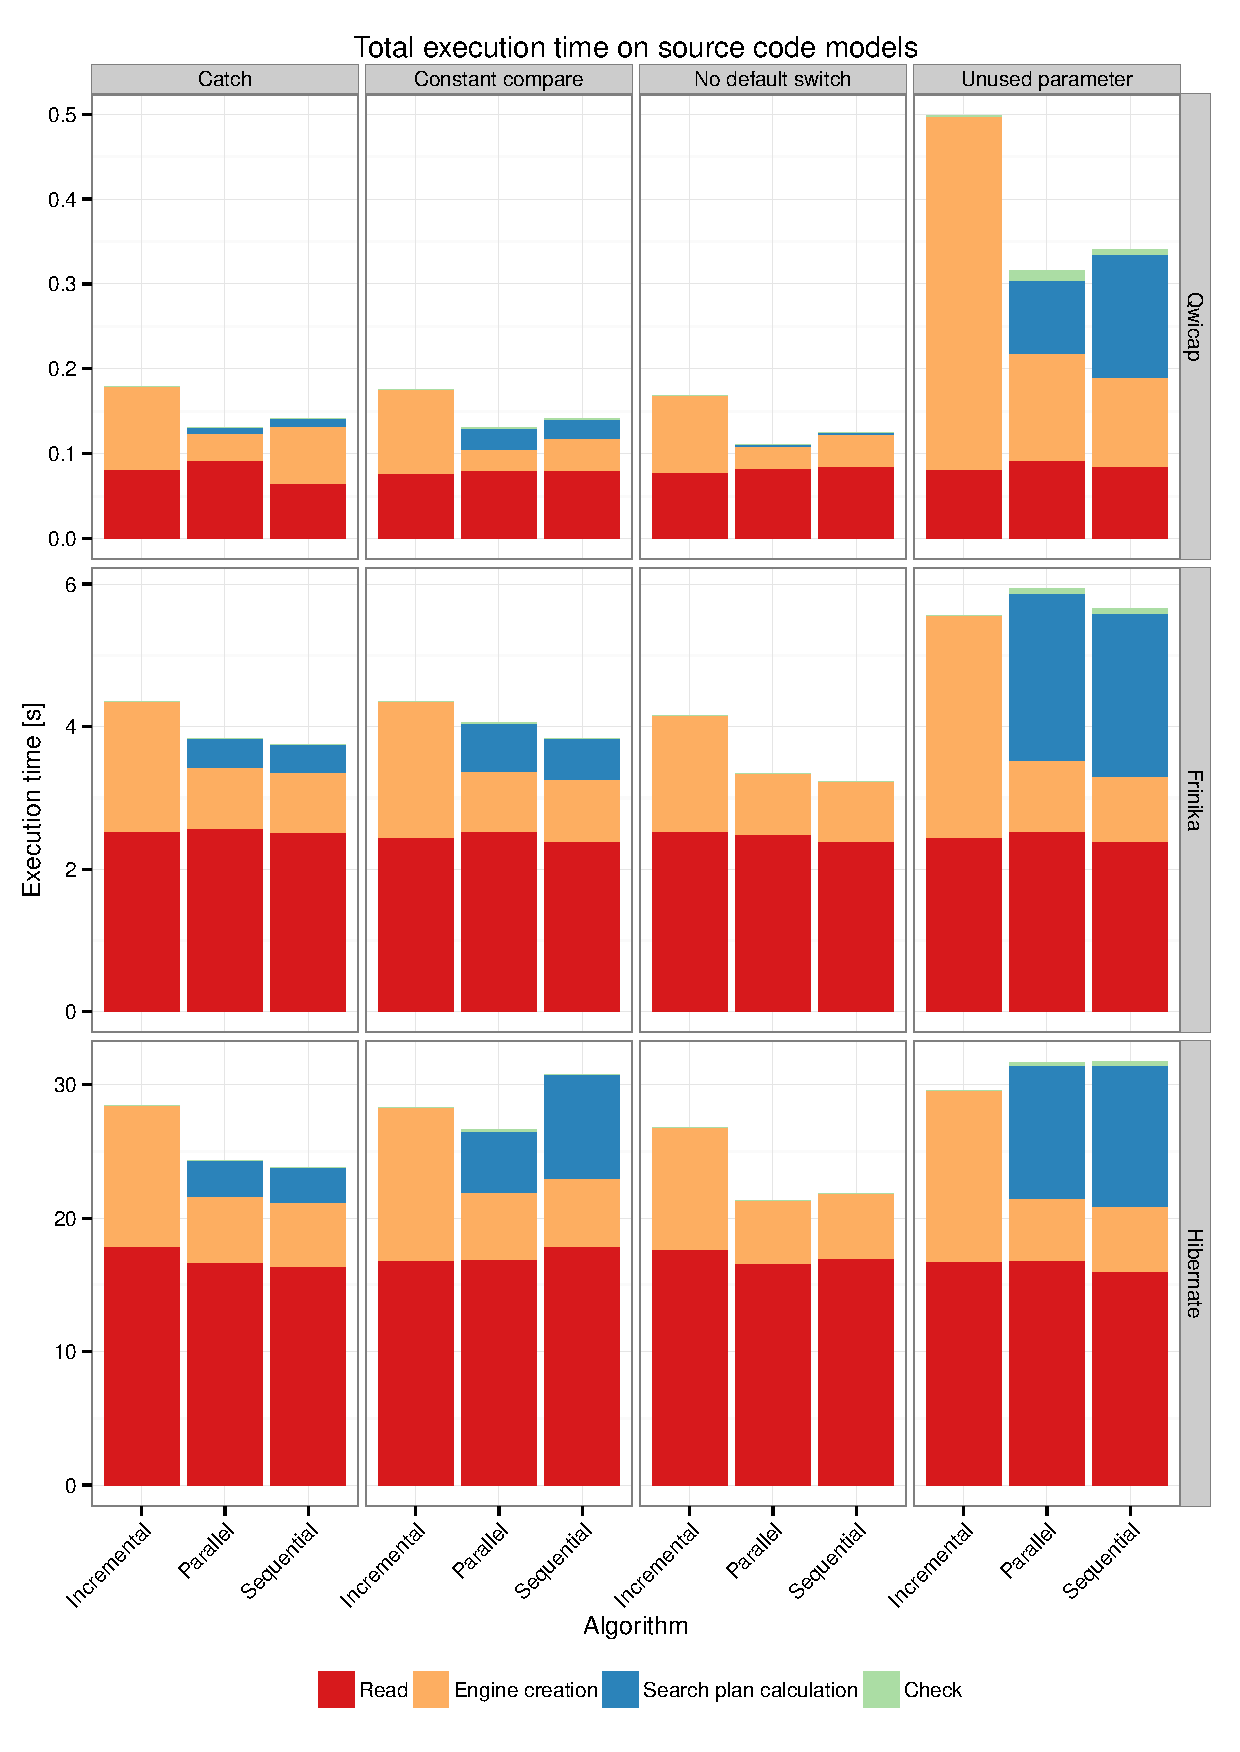
\includegraphics[width=\textwidth]{pdfs/code_model.pdf}
	
	\caption{Measurement results for anti-pattern detection in ASGs}
	\label{fig:csmr-measurements}
\end{figure}


In the Read phase, loading the model takes significant amount of time. In case of large models this is the longest task, but for smaller sizes it is still comparable to engine creation. This complies with the fact that engine creation involves indexing the model elements, and for the Rete algorithm, also building the Rete network based on the index. This also explains why it takes multiple times more, according to the measurements, to finish the engine creation phase for the incremental algorithm.

For the search plan calculation phase, however, unexpectedly large execution times were encountered. This is the step, when the constraints of the pattern are put into an ordered list that makes up the search plan. The current implementation of the algorithm uses cardinality information of types about the instance model in order to determine the order of the operations. After a more detailed analysis of the relevant module, it turned out, that the base indexer has a fairly suboptimal implementation for this part. The method \texttt{countTuples(IInputKey key, Tuple seed)} in \texttt{EMFQueryRuntimeContext} currently returns the result of the \texttt{size()} method called on the result of \texttt{baseIndex.getAllInstances(eClass)}. The already existing implementation of the \texttt{getAllInstances(EClass type)} method of the \texttt{NavigationHelperImpl} class is included in \autoref{lst:getAllInstances}.


\lstset{escapeinside={(*@}{@*)}}
\begin{figure}[!htp]
	\listingjava{getAllInstances}{The implementation of the \texttt{getAllInstances} method}
\end{figure}

This method, as its name advices, returns a collection of all objects of a given type. If we inspect the implementation, in line \autoref{line:newset}, a new \texttt{Set} is instantiated. All subtypes of the given type are collected in line \autoref{line:subtypes}. Between line \autoref{line:subtypes-begin} and line \autoref{line:subtypes-end} all instances of all subtypes are added to \texttt{retSet}, if there were any. In line \autoref{line:instances} all direct instances of the given type are added to the set containing the collected subtype instances. Finally, in \autoref{line:return} \texttt{retSet} is returned. According to our measurements, adding approximately 100,000 elements to an empty set, then calling \texttt{size()} takes about $20$~ms on the computer, on which the performance evaluation was carried out. For these cardinality information are not cached, if it is needed multiple times, the same gathering of elements is carried out again. It also turned out, that the planner in many cases does ask for cardinality information several times for a type.

An important observation is that generally the execution of Check phase may require orders of magnitude less time than other steps. In case of the Rete algorithm this step consists of only returning a copy of a collection in which matches are stored, because it is already prepared by the time the Rete network is built. The local search-based algorithm, however, computes the matches in this final phase of measurement. Thanks to the efficient, model sensitive search plan, which is calculated in the preceding phase, the search for matches is done under a few milliseconds for most cases. We experienced slightly notable durations for the largest used model, Hibernate. In this case the matcher for \emph{Constant compare} and \emph{Unused parameter} patterns worked several hundred milliseconds to compute matches. It is also important to add, that these patterns are considered to be more complex than \emph{Catch} and \emph{No default switch}.

The results also shed light on the shortcomings of the current search parallelization. The implementation creates a thread pool with $c$ threads, where $c$ equals the number of currently available cores of the CPU. Then, the parallelization starts when the search execution reaches the first extend operation, where the potential substitutions are divided between the threads. The creation of a thread pool and distributing the work among threads seemingly imposes some overhead, as it was foreseen in \autoref{sec:advantages-weaknesses}. 

%Also, as it was covered in \autoref{sec:advantages-weaknesses}, at the point of substitution of a value it is not known, how much time will it take to calculate all possible matches. For this reason the distribution of the values among threads may cause uneven workload among executors. However, to get all results all executor thread should finish to be able to create a unified collection of matches.

To decide which algorithm should be used in a certain scenario depends on several circumstances. According to the results, we can estimate the number of runs, where the Rete algorithm outperforms the local search-based one in runtime. If we were to match the \emph{Catch} problem against the model \emph{Frinika} only once, it would take $2.535 + 1.813 + 0 + 0.0017 = 4.3497$~seconds with the incremental algorithm. The same scenario would took $ 2.512 + 0.842 + 0.400 + 0.0009 = 3.7549 $~seconds for the sequential local search-based algorithm. However, if we increased the number of runs on a loaded model with an already created engine, each additional run after the first one would took only $ 0.0017 $~seconds with Rete, and $ 0.4009 $~seconds with the current implementation of the sequential local search-based version. From these data, we can obtain a run count threshold, for which incremental algorithm is more beneficial with respect to execution time. This run threshold $r$ comes from the equation 
$$ 2.535 + 1.813 + r \cdot 0.0017 = 2.512 + 0.842 + r \cdot (0.400 + 0.0009), $$
and it yields $ r \approx 2.5 $. So it means, if we run the same anti-pattern detection several times on the model only one or two times, it is worth using local search, in other cases Rete will finish faster. If we apply the above calculations for the measurement results of \emph{No default switch}, we get a threshold $r \approx 1546.7$. However, we have to remark three important factors regarding the above calculations:

\begin{itemize}
	\item Rete network update times are neglected in this calculation, for they are assumed to be minimal for small model changes.
	\item Currently the search plan calculation is highly ineffective due to a shortcoming in the implementation of the base indexer. If this problem were fixed, the time needed for plan calculation for local search would notably drop.
	\item In these cases the memory bounds were not a limitation.
	\item Search plans are not cached for later execution.
\end{itemize}

\section{Running the Train Benchmark}
\label{sec:performance-evaluation-tb}

Train Benchmark is a benchmarking framework aiming to test query evaluation performance of model-driven engineering tools~\cite{trainbenchmark}. This evaluation is carried out by matching the same patterns against several models with growing sizes. For this purpose Train Benchmark has a model generator component that creates synthetic models for a given size range. It also provides predefined patterns to match against the generated models, for which basic complexity information are included in \autoref{tab:tb-pattern-complexities}. For detailed description of the models provided by the generator and the patterns, please refer to the cited technical report above.


 \begin{table}[ht]
 	\centering
 	\begin{tabular}{l|ccc}
 		\hline
 		Pattern & Variables & Constraints & Pattern calls \\
 		\hline
		 ConnectedSegments & 7 & 7 & 0 \\
		 RouteSensor & 4 & 4 & 1 \\
		 SemaphoreNeighbor & 7 & 8 & 1 \\
		 SwitchSet & 4 & 7 & 0 \\
 		\hline
 	\end{tabular}
 	\caption{Train Benchmark pattern names and complexities}
 	\label{tab:tb-pattern-complexities}
 \end{table}



In our case we used this framework to test the scalability of the pattern matching algorithms on the benchmark scenario depicted in \autoref{fig:measurement-workflow}. We ran these measurements on a virtual machine with the following hardware configuration:

\begin{itemize}
	\item CPU: Intel$\circledR$ Xeon$\circledR$ CPU E5-2630L v2 @ 2.40GHz (12 cores)
	\item Memory: 32 GB DDR3 @ 1600 MHz
	\item SSD: Intel Corporation 82371SB PIIX3 IDE [Natoma/Triton II]
\end{itemize}

We used Java\texttrademark~SE Runtime Environment (build 1.8.0\_66-b17), and ran the JVM without extra parameters, which means the heap size limit was 1 GB.

Benchmarking memory consumption is a non-trivial issue in case of managed environments like Java. For this reason we chose a limit for the maximum heap size. From this limit we will not know the exact amount of memory needed, an \emph{out of memory error} can indicate that the program could not fit in the available size. This strategy can be used to decide which algorithm needs more memory than others.

The performance characteristics were similar to what we described previously in \autoref{sec:performance-evaluation}. The search plan generation times for the patterns of Train Benchmark, depicted in \autoref{fig:tb-calc-search-plan}, were increasing with model size (in the diagram both axes are logarithmic). This also leads to the conclusion that obtaining type cardinality information depends on model sizes. The diagram also shows that search plan calculation for different patterns for the same model size take time based on the complexity of the pattern.


\begin{figure}[htpb]
	\centering
	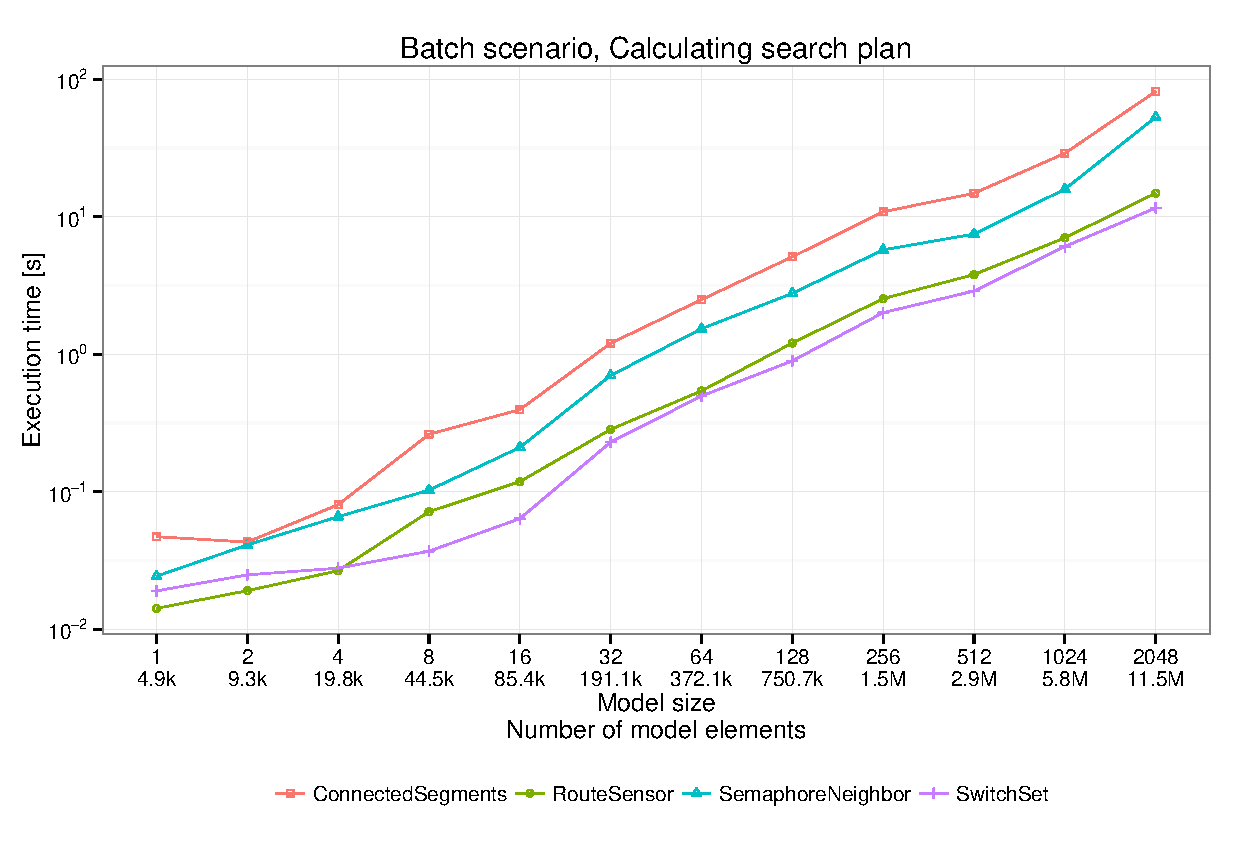
\includegraphics[width=\linewidth]{pdfs/Batch-Calculating-search-plan.pdf}
	
	\caption{Search plan calculation times for different patterns}
	\label{fig:tb-calc-search-plan}
\end{figure}

On the synthesized models of Train Benchmark, we measured mostly linear characteristics for both the sequential and the parallel local search-based pattern matching. The results are depicted in \autoref{fig:tb-check} (again, note the logarithmic axes in the diagram). In this cases, we can observe almost immediate retrieval of results in case of Rete for every pattern. However, for the local search based-pattern matching solutions both scale up in a linear way with the model sizes. We can see that the parallel version of the implementation has an overhead compared to the sequential solution, by comparing the check times needed for small model sizes. This overhead, however, may pay off, since in case of large models the parallel version completes faster.

The benchmark also showed that the incremental algorithm is more constrained by memory than local search-based approaches. While running the benchmark with \emph{ConnectedSegments} on model scale 2048, the measurement was terminated by an out of memory error, showing that the Rete network grew too large in this case.

\begin{figure}[htpb]
	\centering
	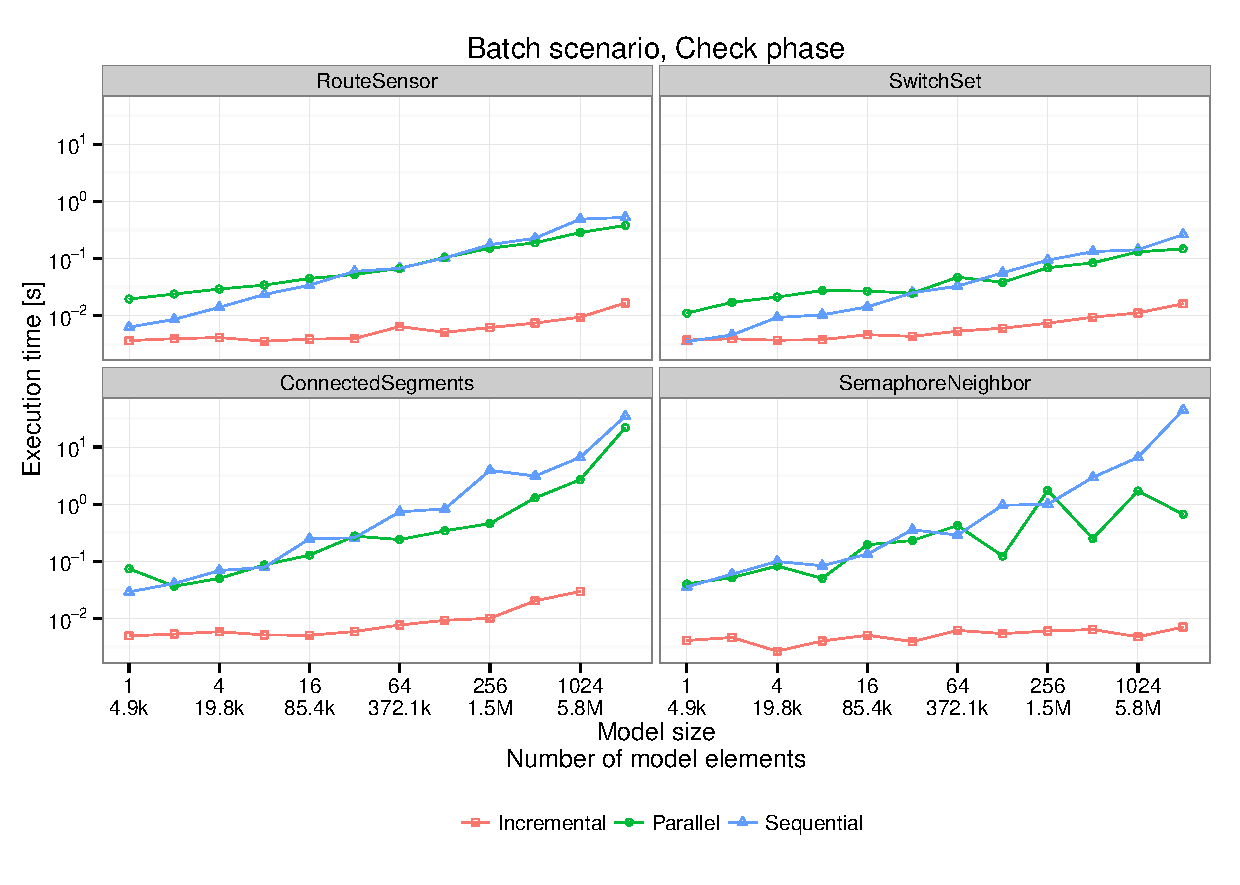
\includegraphics[width=\linewidth]{pdfs/Batch-Check-phase.pdf}
	\caption{Times needed for the Check phase}
	\label{fig:tb-check}
\end{figure}


The rest of the diagrams and tables, which contain the evaluation results of the benchmark, are included in \autoref{appendix:trainbenchmark-results} in the Appendix.

\section{Evaluation summary}

Based on the performed measurements, we came to the conclusion that the \emph{incremental Rete algorithm} runs significantly slower for the first time, compared to the implemented local search-based approach. It also requires more memory for execution. However, we recommend to use this algorithm despite these extra requirements if the same pattern should be matched against the model multiple times consecutively, and if sufficient amount of memory is available.

The sequential local search-based solution has lower memory requirement in many cases, compared to Rete. If the pattern matching is a one-time task, and the cardinality information about the model elements is available, then this is the recommended algorithm.


The parallel local search-based approach differs from the sequential version only in search execution. It has an initial overhead, but for large models it is more preferable in cases where local search should be used.

%2 oldal


%\begin{figure}
%	\centering
%	\subfloat{%
%		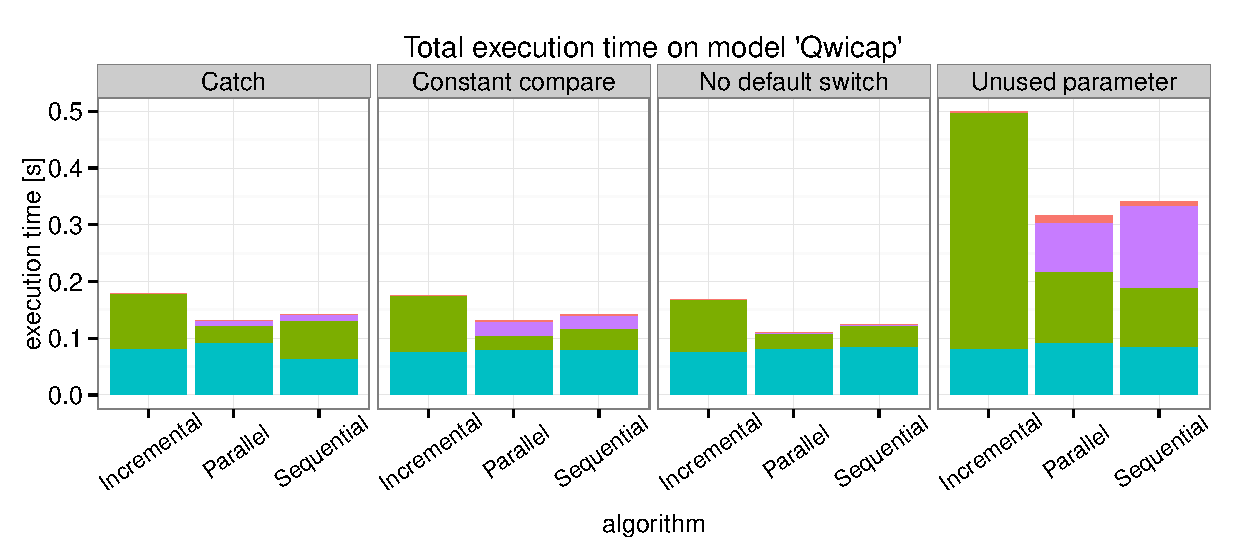
\includegraphics[width=\linewidth]{pdfs/qwicap_resized.pdf}
%	}\par
%	\subfloat{%
%		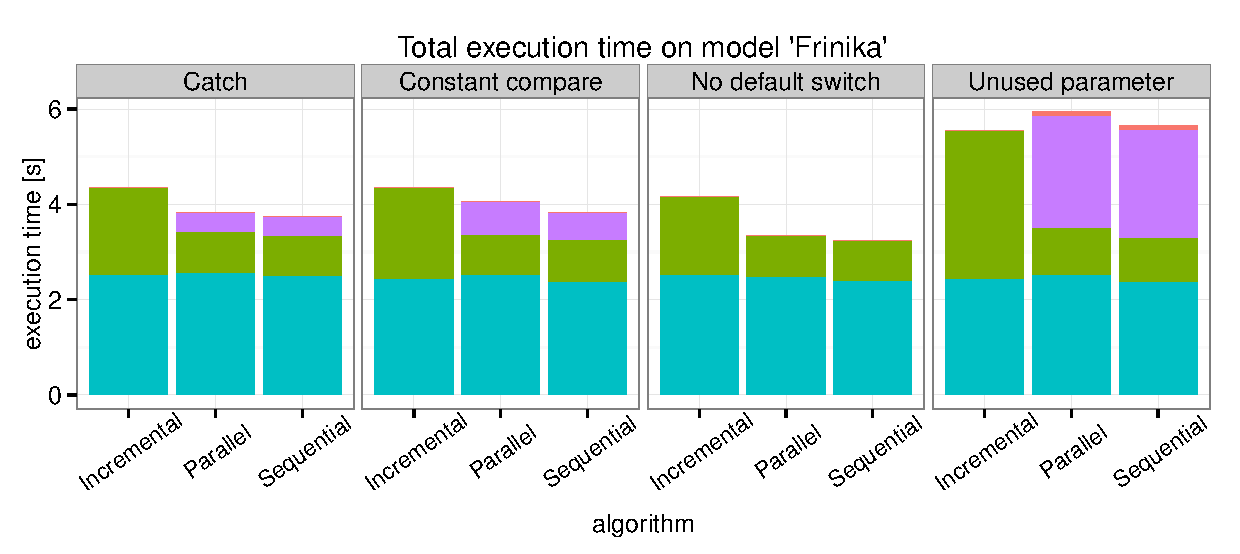
\includegraphics[width=\linewidth]{pdfs/frinika_resized.pdf}
%	}\par        
%	\subfloat{%
%		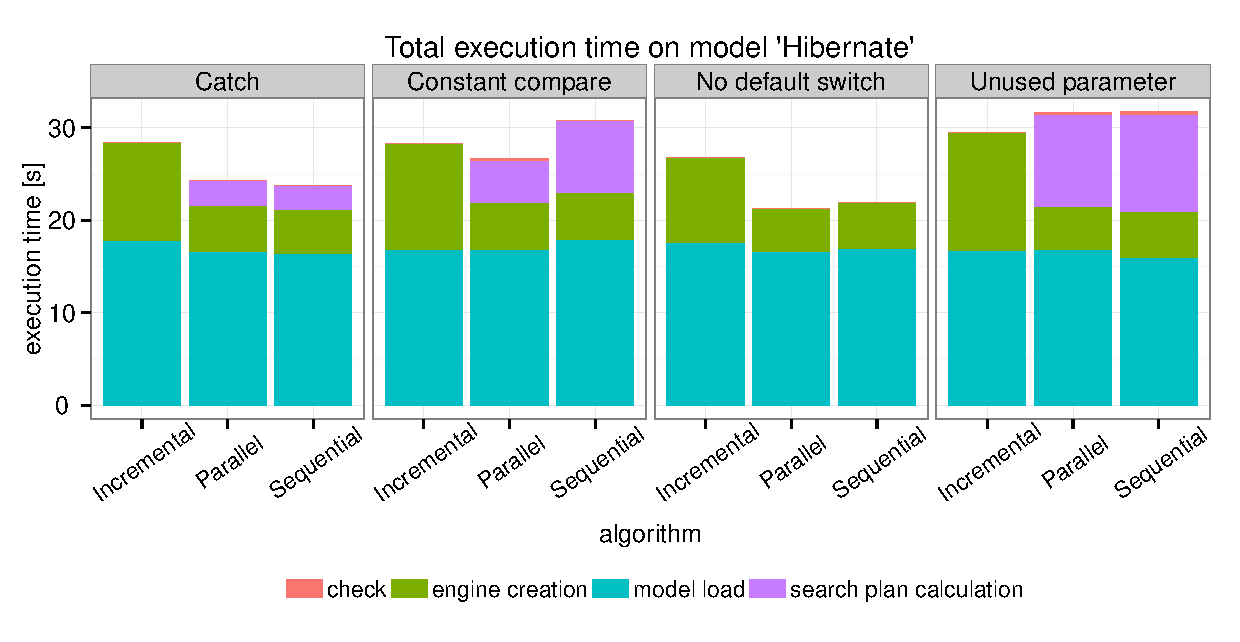
\includegraphics[width=\linewidth]{pdfs/hibernate_resized.pdf}
%	}
%	\caption{Measurement results for anti-pattern detection in ASGs}
%	\label{fig:csmr-measurements}
%\end{figure}




%\clearpage
%\begin{figure}[hp]
%	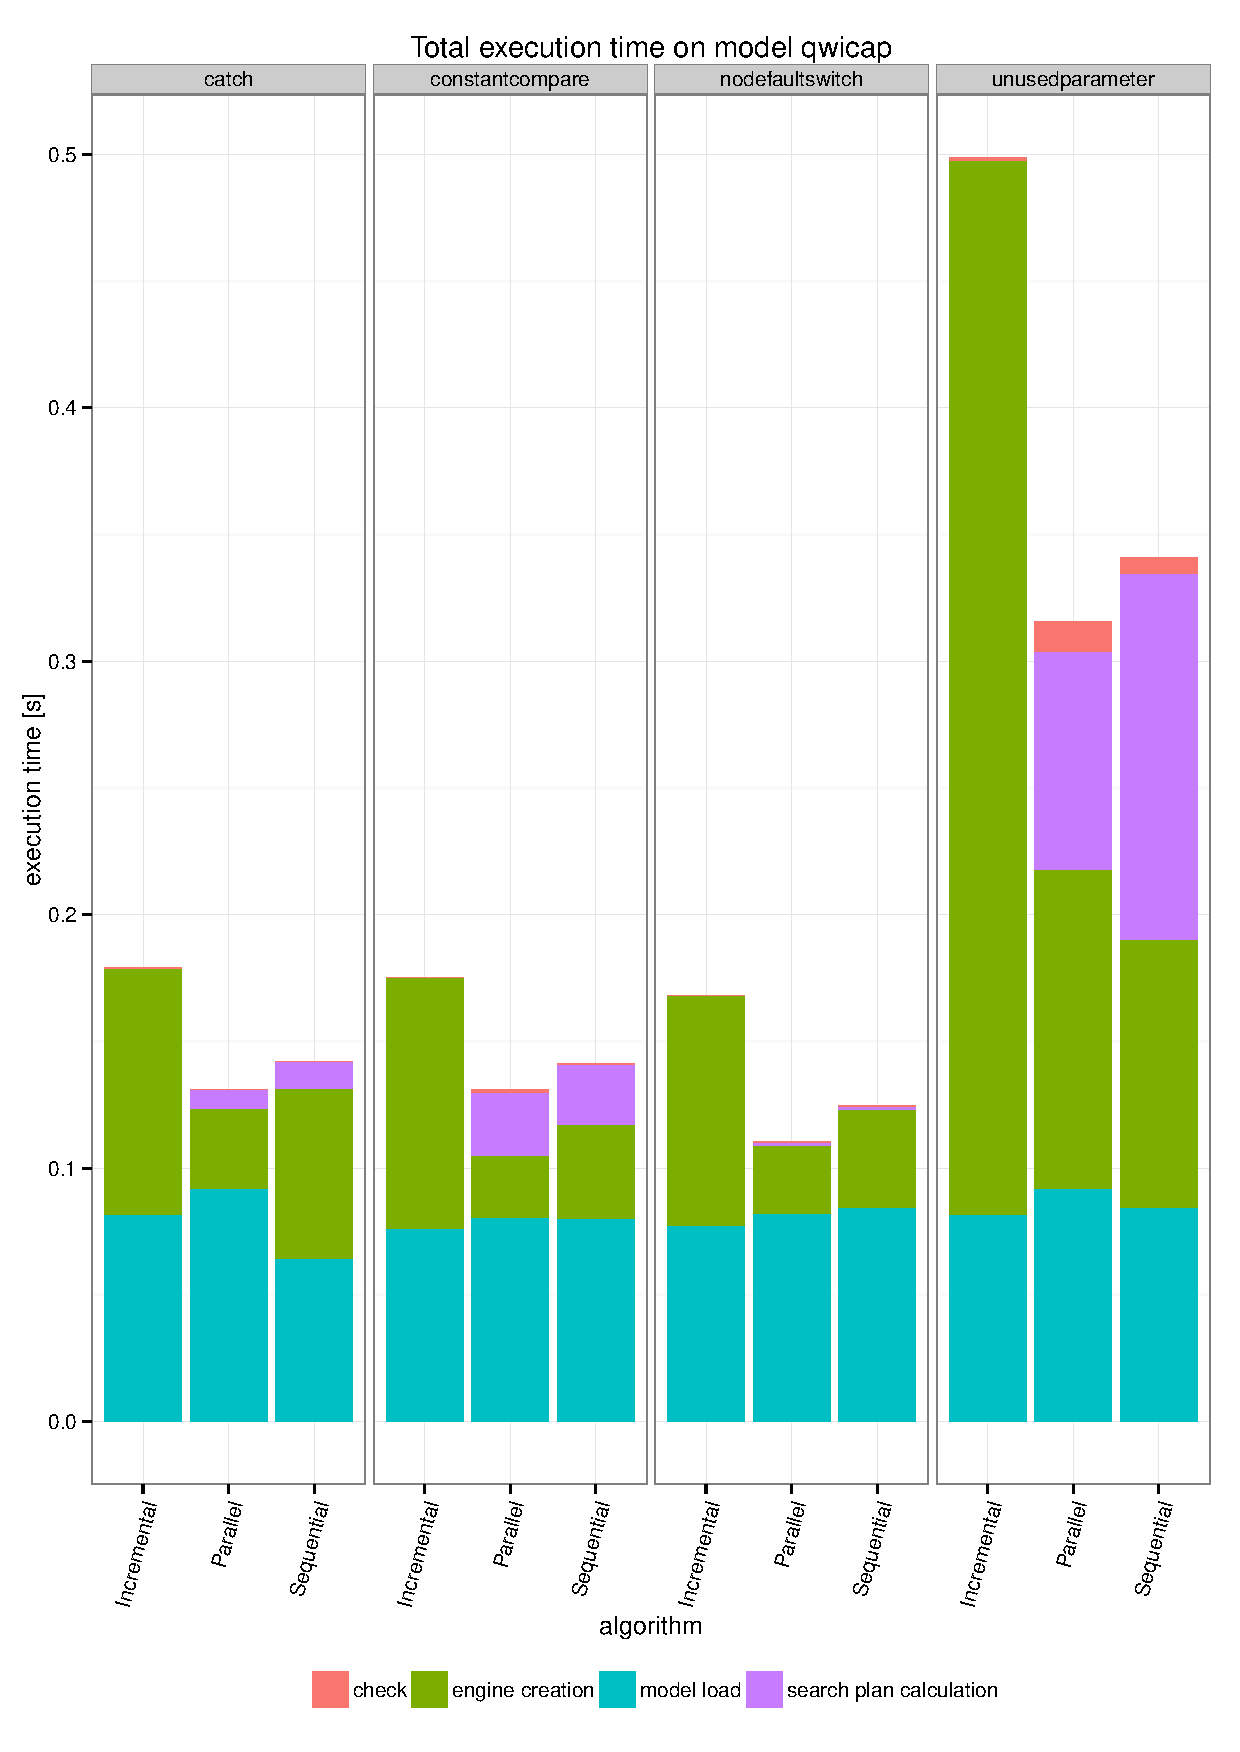
\includegraphics[width=\linewidth]{pdfs/qwicap.pdf}
%\end{figure}
%\begin{figure}[hp]
%	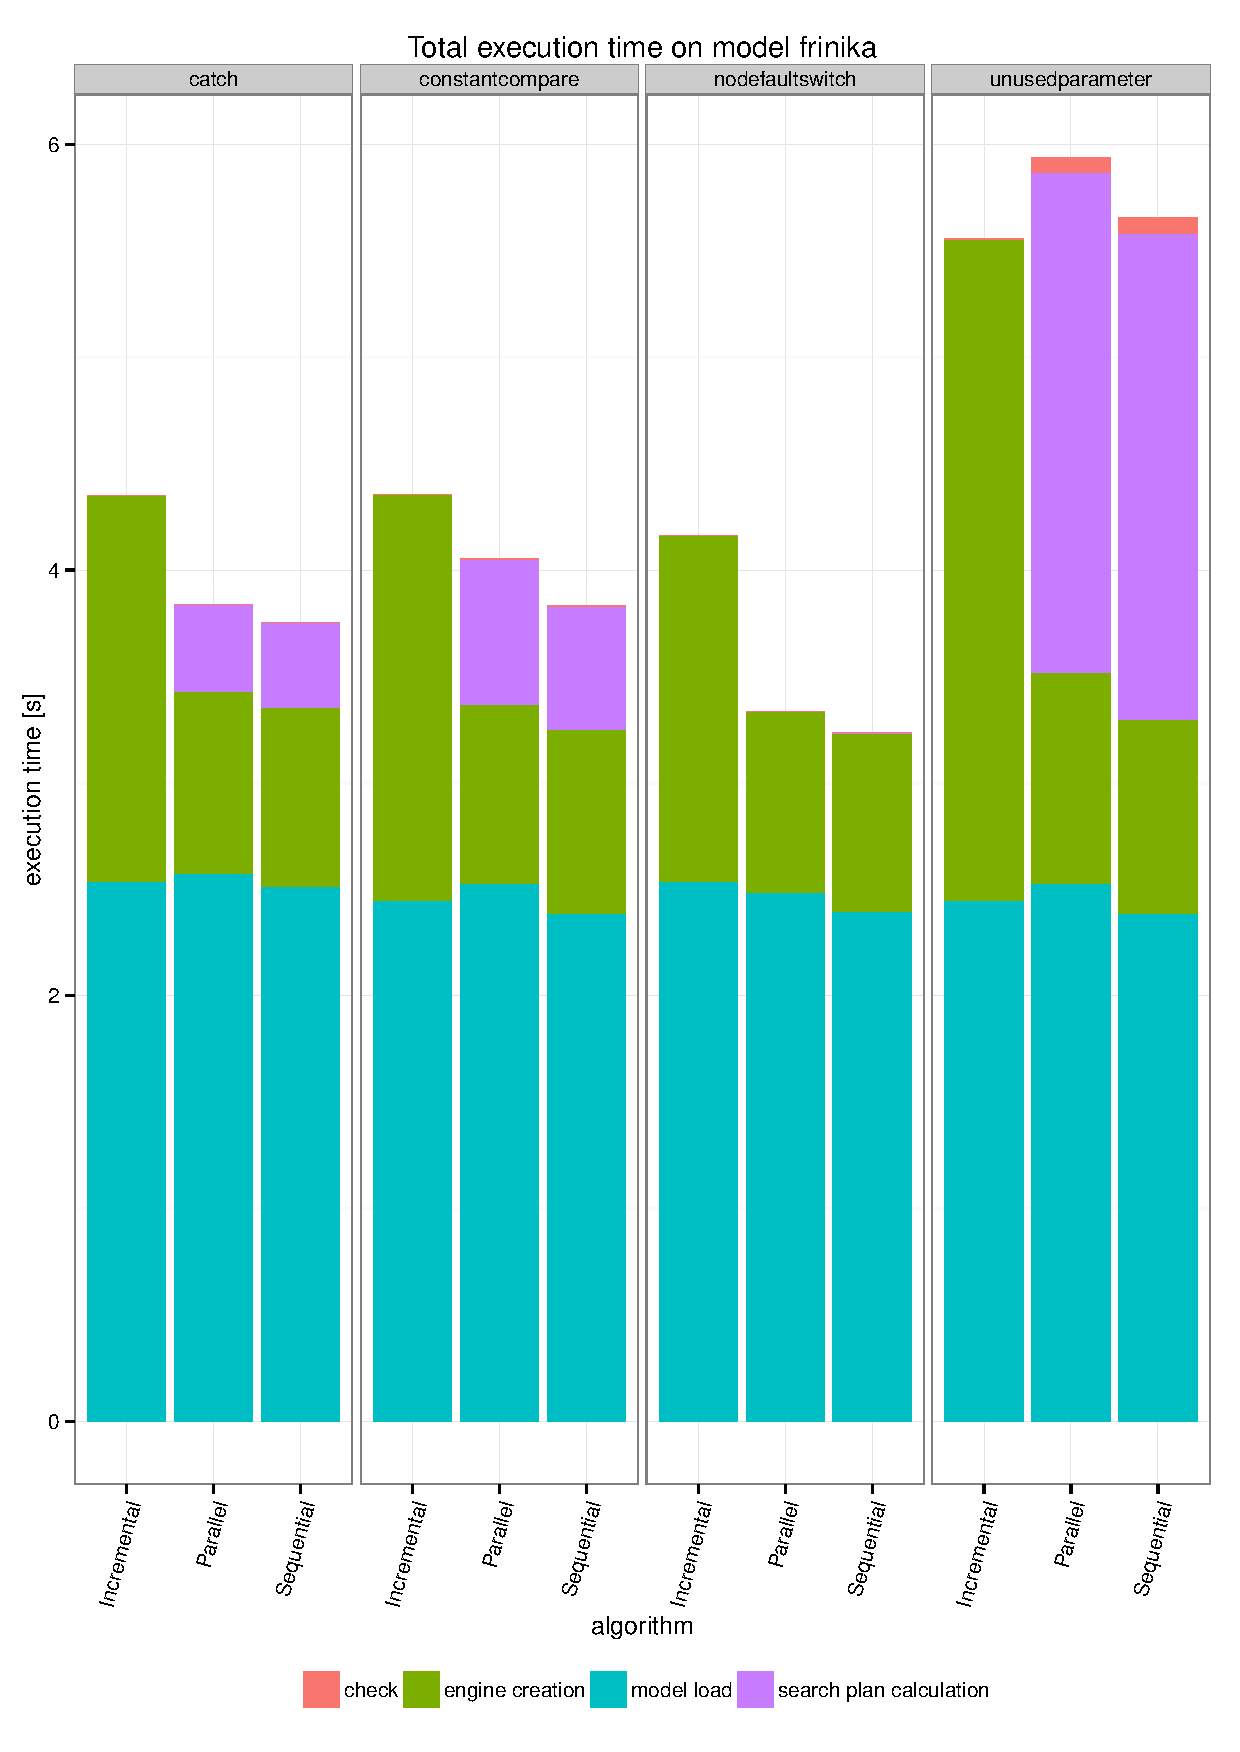
\includegraphics[width=\linewidth]{pdfs/frinika.pdf}
%\end{figure}
%\begin{figure}[hp]
%	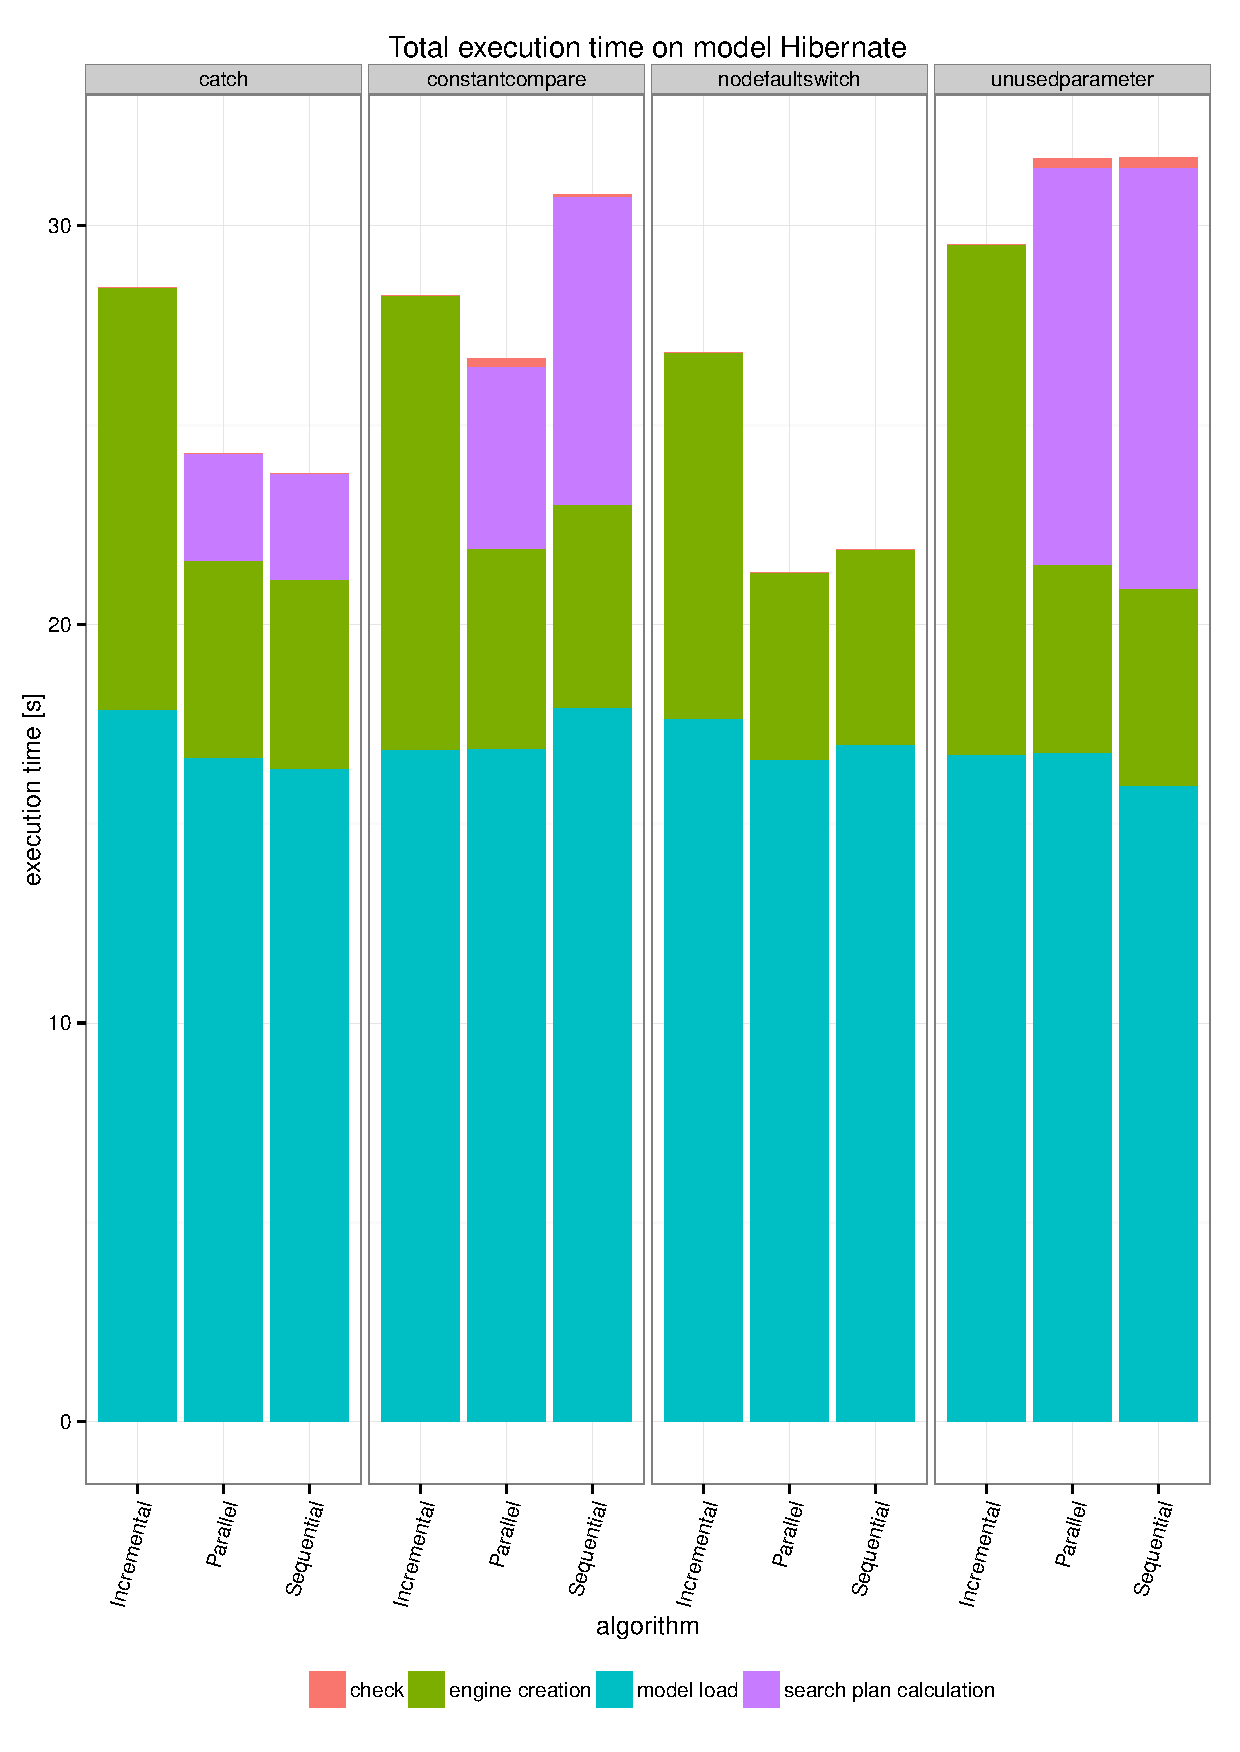
\includegraphics[width=\linewidth]{pdfs/hibernate.pdf}
%\end{figure}